\documentclass[aspectratio=169,11pt]{beamer}

\usetheme{AnnArbor}
\usecolortheme{dolphin}
\usefonttheme{professionalfonts}
\setbeamertemplate{navigation symbols}{}
\setbeamertemplate{caption}[numbered]

\usepackage{fontspec}
\setsansfont{DejaVu Sans}
\setmonofont{DejaVu Sans Mono}
\usepackage{amsmath,amssymb}
\usepackage{booktabs}
\usepackage{array}
\usepackage{tikz}
\usetikzlibrary{arrows.meta,positioning,shapes.geometric,fit}
\usepackage{hyperref}
\hypersetup{colorlinks=true,linkcolor=blue,urlcolor=blue}

\title[DBMS]{Database Management Systems and MySQL}
\subtitle{Course Roadmap \& Learning Overview}
\author{Vu Duc Minh}
\institute{National Economics University, Hanoi, Vietnam}
\date{\today}

\definecolor{dbblue}{RGB}{20,74,135}
\definecolor{dblight}{RGB}{232,242,255}
\definecolor{dbgreen}{RGB}{28,120,90}
\definecolor{dborange}{RGB}{210,120,30}

\setbeamercolor{structure}{fg=dbblue}
\setbeamercolor{title}{fg=white,bg=dbblue}
\setbeamercolor{frametitle}{fg=dbblue}
\setbeamercolor{block title}{fg=white,bg=dbblue}
\setbeamercolor{block body}{bg=dblight,fg=black}

\newcommand{\kw}[1]{\textcolor{dbblue}{\textbf{#1}}}
\newcommand{\smallgap}{\vspace{0.4em}}

\begin{document}

%------------------------------------------------
\begin{frame}
  \titlepage
\end{frame}

%------------------------------------------------
\begin{frame}{Course Learning Objectives}
By the end of this course, students should be able to:
\begin{itemize}
  \item Explain the role of \kw{databases} and \kw{DBMSs} in information systems.
  \item Design conceptual data models using the \kw{ER/EER model}.
  \item Map ER models to \kw{relational schemas} and analyze keys and functional dependencies.
  \item Apply \kw{normalization} to reduce redundancy and improve data consistency.
  \item Use \kw{MySQL} to administer, query, optimize, and program database systems.
\end{itemize}
\end{frame}

%------------------------------------------------
\begin{frame}{Course Big Picture}
\centering
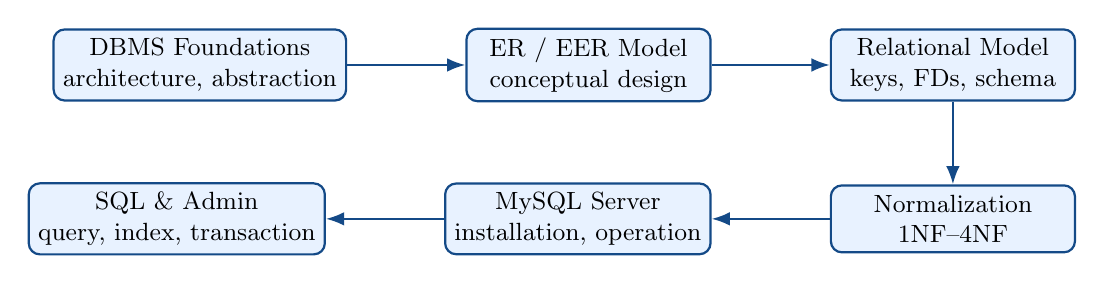
\begin{tikzpicture}[
  node distance=1.05cm and 1.5cm,
  box/.style={rounded corners, draw=dbblue, thick, fill=dblight, minimum width=3.1cm, minimum height=0.85cm, align=center, font=\small},
  arr/.style={-Latex, thick, draw=dbblue}
]
\node[box] (intro) {DBMS Foundations\\architecture, abstraction};
\node[box, right=of intro] (er) {ER / EER Model\\conceptual design};
\node[box, right=of er] (rel) {Relational Model\\keys, FDs, schema};
\node[box, below=of rel] (norm) {Normalization\\1NF--4NF};
\node[box, left=of norm] (mysql) {MySQL Server\\installation, operation};
\node[box, left=of mysql] (sql) {SQL \& Admin\\query, index, transaction};
\draw[arr] (intro) -- (er);
\draw[arr] (er) -- (rel);
\draw[arr] (rel) -- (norm);
\draw[arr] (norm) -- (mysql);
\draw[arr] (mysql) -- (sql);
\end{tikzpicture}

\smallgap
\textit{Main idea: move from data modeling to database implementation and data exploitation with MySQL.}
\end{frame}

%------------------------------------------------
\section{Introduction}
\begin{frame}{Part 1: Introduction to DBMS}
\begin{block}{Main topics}
\begin{itemize}
  \item Databases and database management systems.
  \item Why DBMSs are needed in real-world information systems.
  \item One-tier, two-tier, and three-tier architectures.
  \item Data abstraction and data independence.
  \item Schema, instance, and data models.
\end{itemize}
\end{block}

\begin{alertblock}{Guiding question}
Why should a business application avoid storing important data in separate unmanaged files?
\end{alertblock}
\end{frame}

%------------------------------------------------
\begin{frame}{What Problems Does a DBMS Solve?}
\begin{columns}[T,onlytextwidth]
\column{0.48\textwidth}
\begin{block}{Without a DBMS}
\begin{itemize}
  \item Duplicate data and weak control.
  \item Difficulty maintaining consistency.
  \item Manual security and access control.
  \item Hard backup, recovery, and scaling.
\end{itemize}
\end{block}
\column{0.48\textwidth}
\begin{block}{With a DBMS}
\begin{itemize}
  \item Centralized data management.
  \item Data integrity constraints.
  \item SQL-based querying.
  \item Transactions, security, and backup support.
\end{itemize}
\end{block}
\end{columns}
\end{frame}

%------------------------------------------------
\section{ER Model}
\begin{frame}{Part 2: Entity Relationship Model}
\begin{block}{Role}
The ER model describes data at the \kw{conceptual} level before it is translated into relational database tables.
\end{block}

\begin{columns}[T,onlytextwidth]
\column{0.32\textwidth}
\textbf{Entities}\\
Customers, orders, products.
\column{0.32\textwidth}
\textbf{Attributes}\\
Customer ID, order date, selling price.
\column{0.32\textwidth}
\textbf{Relationships}\\
A customer places orders; an order contains products.
\end{columns}

\smallgap
\begin{alertblock}{Practice}
Identify entities, attributes, keys, and relationships for a small sales system.
\end{alertblock}
\end{frame}

%------------------------------------------------
\begin{frame}{From Business Requirements to ERD}
\centering
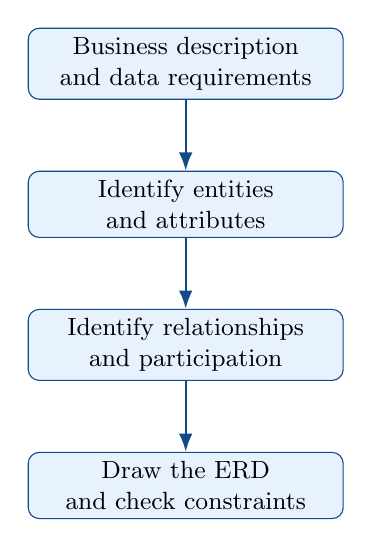
\begin{tikzpicture}[
  node distance=0.9cm,
  process/.style={draw=dbblue, rounded corners, fill=dblight, align=center, minimum width=4.0cm, minimum height=0.82cm, font=\small},
  arr/.style={-Latex, thick, draw=dbblue}
]
\node[process] (req) {Business description\\and data requirements};
\node[process, below=of req] (entity) {Identify entities\\and attributes};
\node[process, below=of entity] (rel) {Identify relationships\\and participation};
\node[process, below=of rel] (erd) {Draw the ERD\\and check constraints};
\draw[arr] (req) -- (entity);
\draw[arr] (entity) -- (rel);
\draw[arr] (rel) -- (erd);
\end{tikzpicture}
\end{frame}

%------------------------------------------------
\section{Relational Model}
\begin{frame}{Part 3: Relational Model and Functional Dependencies}
\begin{block}{Main topics}
\begin{itemize}
  \item Relation, attribute, tuple, and relational schema.
  \item Super key, candidate key, primary key, and foreign key.
  \item Mapping from ER model to relational model.
  \item Functional dependency: determinant and dependent attribute.
  \item Attribute closure and schema design strategies.
\end{itemize}
\end{block}

\begin{exampleblock}{Example}
If \texttt{StudentID} uniquely determines \texttt{StudentName}, then:
\[
\texttt{StudentID} \rightarrow \texttt{StudentName}.
\]
\end{exampleblock}
\end{frame}

%------------------------------------------------
\begin{frame}{Mapping ER Models to Relations}
\begin{columns}[T,onlytextwidth]
\column{0.52\textwidth}
\begin{itemize}
  \item Each strong entity usually becomes a table.
  \item The entity key becomes the table primary key.
  \item A one-to-many relationship is usually represented by a foreign key on the many side.
  \item A many-to-many relationship is usually converted into an associative table.
\end{itemize}
\column{0.44\textwidth}
\begin{block}{Example}
\texttt{Customer(CustomerID, Name)}\\
\texttt{Order(OrderID, OrderDate, CustomerID)}
\end{block}
\end{columns}

\begin{alertblock}{Design check}
A good design preserves business meaning, keys, and relationship constraints.
\end{alertblock}
\end{frame}

%------------------------------------------------
\section{Normalization}
\begin{frame}{Part 4: Normalization}
\begin{block}{Goal}
Normalization reduces data redundancy and prevents update, insertion, and deletion anomalies.
\end{block}

\begin{center}
\begin{tabular}{>{\bfseries}p{0.16\textwidth} p{0.72\textwidth}}
\toprule
1NF & Each cell stores an atomic value; repeating groups are removed.\\
2NF & No partial dependency on part of a composite key.\\
3NF & No transitive dependency among non-key attributes.\\
4NF & Independent multivalued dependencies are handled properly.\\
\bottomrule
\end{tabular}
\end{center}
\end{frame}

%------------------------------------------------
\begin{frame}{Normalization Thinking}
\centering
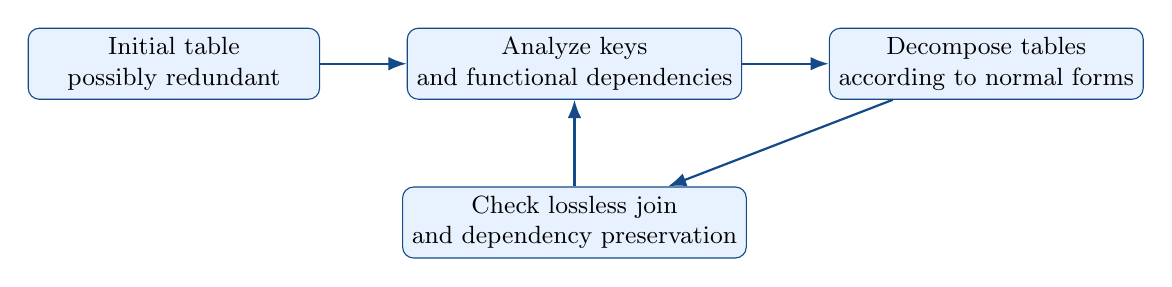
\begin{tikzpicture}[
  node distance=1.1cm,
  box/.style={draw=dbblue, rounded corners, fill=dblight, align=center, minimum width=3.7cm, minimum height=0.85cm, font=\small},
  arr/.style={-Latex, thick, draw=dbblue}
]
\node[box] (raw) {Initial table\\possibly redundant};
\node[box, right=of raw] (fd) {Analyze keys\\and functional dependencies};
\node[box, right=of fd] (decomp) {Decompose tables\\according to normal forms};
\node[box, below=of fd] (check) {Check lossless join\\and dependency preservation};
\draw[arr] (raw) -- (fd);
\draw[arr] (fd) -- (decomp);
\draw[arr] (decomp) -- (check);
\draw[arr] (check) -- (fd);
\end{tikzpicture}
\end{frame}

%------------------------------------------------
\section{MySQL Server}
\begin{frame}{Part 5: MySQL Server}
\begin{block}{Implementation topics}
\begin{itemize}
  \item Introduction to MySQL and its tool ecosystem.
  \item Installing MySQL Server and MySQL Workbench on Windows.
  \item Connecting through command line and VS Code.
  \item Starting, stopping, and restarting the MySQL service.
  \item Loading the \texttt{classicmodels} sample database.
  \item Storage engines, option files, system variables, and the data directory.
\end{itemize}
\end{block}
\end{frame}

%------------------------------------------------
\begin{frame}[fragile]{Basic MySQL Operations}
\begin{block}{Create and select a database}
\begin{verbatim}
CREATE DATABASE shop_db
  CHARACTER SET utf8mb4
  COLLATE utf8mb4_unicode_ci;

USE shop_db;
SHOW TABLES;
\end{verbatim}
\end{block}

\begin{alertblock}{Safety checklist}
Before running \texttt{DROP DATABASE} or \texttt{DROP TABLE}, verify the environment, verify the database/table name, and make sure an appropriate backup exists for important data.
\end{alertblock}
\end{frame}

%------------------------------------------------
\section{SQL}
\begin{frame}{Part 6: SQL Statements in MySQL}
\begin{columns}[T,onlytextwidth]
\column{0.48\textwidth}
\begin{block}{Data Definition}
\begin{itemize}
  \item Data types.
  \item \texttt{CREATE TABLE}.
  \item Constraints.
  \item \texttt{ALTER}, \texttt{RENAME}, \texttt{DROP}, \texttt{TRUNCATE}.
\end{itemize}
\end{block}
\column{0.48\textwidth}
\begin{block}{Querying Data}
\begin{itemize}
  \item Basic \texttt{SELECT}.
  \item \texttt{JOIN}, \texttt{GROUP BY}, \texttt{HAVING}.
  \item Subqueries and CTEs.
  \item Set operations and window functions.
\end{itemize}
\end{block}
\end{columns}
\end{frame}

%------------------------------------------------
\begin{frame}[fragile]{Sample SELECT Query}
\begin{block}{Total revenue by customer}
\begin{verbatim}
SELECT c.customerName,
       SUM(od.quantityOrdered * od.priceEach) AS revenue
FROM customers c
JOIN orders o ON c.customerNumber = o.customerNumber
JOIN orderdetails od ON o.orderNumber = od.orderNumber
GROUP BY c.customerNumber, c.customerName
ORDER BY revenue DESC;
\end{verbatim}
\end{block}
\end{frame}

%------------------------------------------------
\begin{frame}{Indexes, Query Optimization, and Transactions}
\begin{block}{Index Optimization}
\begin{itemize}
  \item Create, drop, and inspect indexes.
  \item Composite indexes, unique indexes, prefix indexes, and invisible indexes.
  \item Read \texttt{EXPLAIN} and use index hints when necessary.
\end{itemize}
\end{block}

\begin{block}{Data Modification \& Transactions}
\begin{itemize}
  \item \texttt{INSERT}, \texttt{UPDATE}, \texttt{DELETE}, and advanced data modification.
  \item \texttt{START TRANSACTION}, \texttt{COMMIT}, \texttt{ROLLBACK}, and \texttt{SAVEPOINT}.
  \item Locking, row locks, metadata locks, and deadlocks.
\end{itemize}
\end{block}
\end{frame}

%------------------------------------------------
\section{Programmability}
\begin{frame}{Part 7: Views, Procedures, Functions, Triggers, and Events}
\begin{block}{Core idea}
These database objects package processing logic inside the database, reduce repeated application-layer code, and support task automation.
\end{block}

\begin{columns}[T,onlytextwidth]
\column{0.5\textwidth}
\begin{itemize}
  \item \kw{View}: packages a query.
  \item \kw{Stored procedure}: packages a processing workflow.
  \item \kw{Stored function}: returns a value.
\end{itemize}
\column{0.5\textwidth}
\begin{itemize}
  \item \kw{Trigger}: runs automatically on INSERT/UPDATE/DELETE.
  \item \kw{Event}: schedules recurring tasks in MySQL.
\end{itemize}
\end{columns}
\end{frame}

%------------------------------------------------
\begin{frame}{Suggested Learning Roadmap}
\centering
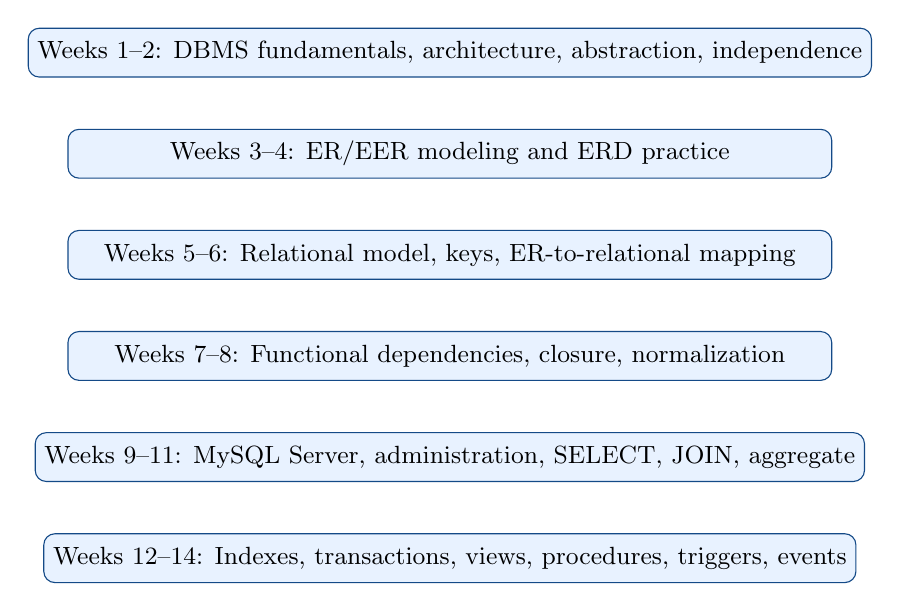
\begin{tikzpicture}[
  node distance=0.65cm,
  week/.style={draw=dbblue, rounded corners, fill=dblight, align=left, minimum width=9.7cm, minimum height=0.62cm, font=\small},
]
\node[week] (w1) {Weeks 1--2: DBMS fundamentals, architecture, abstraction, independence};
\node[week, below=of w1] (w2) {Weeks 3--4: ER/EER modeling and ERD practice};
\node[week, below=of w2] (w3) {Weeks 5--6: Relational model, keys, ER-to-relational mapping};
\node[week, below=of w3] (w4) {Weeks 7--8: Functional dependencies, closure, normalization};
\node[week, below=of w4] (w5) {Weeks 9--11: MySQL Server, administration, SELECT, JOIN, aggregate};
\node[week, below=of w5] (w6) {Weeks 12--14: Indexes, transactions, views, procedures, triggers, events};
\end{tikzpicture}
\end{frame}

%------------------------------------------------
\begin{frame}{Learning Activities and Assessment}
\begin{columns}[T,onlytextwidth]
\column{0.47\textwidth}
\begin{block}{Activities}
\begin{itemize}
  \item Read lecture notes before class.
  \item Complete MySQL and \texttt{classicmodels} labs.
  \item Draw ERDs from business scenarios.
  \item Write queries and explain results.
\end{itemize}
\end{block}
\column{0.47\textwidth}
\begin{block}{Outputs}
\begin{itemize}
  \item ERD and relational schema.
  \item SQL scripts for tables and constraints.
  \item Analytical SQL query set.
  \item Short report on design and optimization.
\end{itemize}
\end{block}
\end{columns}
\end{frame}

%------------------------------------------------
\begin{frame}{Main References}
\begin{itemize}
  \item Carlos Coronel, Steven Morris. \textit{Database Systems: Design, Implementation, and Management}, 14th Edition. Cengage, 2023.
  \item Elvis C. Foster, Shripad Godbole. \textit{Database Systems: A Pragmatic Approach}, 3rd Edition. CRC Press / Taylor \& Francis, 2022.
  \item MySQL Tutorial: practical materials on MySQL, SQL, and advanced topics.
  \item GeeksforGeeks DBMS and SQL tutorials: supplementary topic-based materials.
  \item Roadmap.sh SQL Roadmap: a self-study roadmap for SQL.
\end{itemize}
\end{frame}

%------------------------------------------------
\begin{frame}
\centering
\Huge \textbf{Thank you!}

\vspace{1em}
\Large Questions \& Discussion
\end{frame}

\end{document}
